\documentclass[14pt]{article}

\usepackage{Packages}
\usepackage{Commands}

\begin{document}

\maketitle

\begin{abstract}
В работе изучается модель Изинга на случайном блуждании без самопересечений на квадратной, треугольной, кубической и 4D-гиперкубической решётках, 
в сравнении с родительскими моделями взаимодействующего случайного блуждания без самопересечений и классической модели Изинга на прямоугольной решётке.
С помощью метода Монте-Карло по алгоритму Червя и кластерному алгоритму Вольфа изучены геометрические и магнитные свойства, и
проведено их сравнение с родительскими моделями и между модификациями изучаемой модели в аналогичных условиях.
\end{abstract}



\tableofcontents


\section{Введение}

Модель случайных блужданий без самопересечений (далее - СБС) - одна из наиболее широко изученных моделей из класса линейных полимеров. 
Более того, она является одной из простейших моделей для изучения критического поведения - так, в случае когда модель усложнена наличием взаимодействия между ближайшими узлами цепочки, её фазовый переход оказывается зафиксирован между состояниями её растворителя, и при термическом равновесии системы полученная полимерная цепочка будет схлопнутой в условиях сильного растворителя или вытянутой в слабом растворителе.
Трикритичность данного перехода была описана в работе \cite{Gennes1979}.

Влияние близких связей было широко рассмотрено среди класса моделей магнитного полимера, взаимодействие между узлами которых стало ещё более сложным:
каждый узел обладает спином, а сила взаимодействия между ближайшими узлами стала отдельным параметром. 
Её название - модель Изинга на случайном блуждании без самопересечений.
В работе \cite{Garel1999} был рассмотрен случай, когда она так же обладает переменным внешним полем, и все заключения о её магнитных свойствах были оценены в сравнении с моделью среднего поля.
В то же время влияние геометрических свойств модели на магнитные не до конца ясно и их изучение в некоторых случаях требует статистического подхода.

В предыдущей работе \cite{faizullina2021critical} было определено, что фазовый переход двумерной модели Изинга на CБС
имеет непрерывный характер. 
В этой работе мы продолжаем изучать геометрические свойства данной модели и сравнивать их с её родительскими моделями или модификациями, такими как классическая модель Изинга на регулярной решётке, опредёленная в работе \cite{selke2006critical}, и взаимодействующее случайное блуждание без самопересечений в соответствующих критических областях. 
Мы предполагаем, что модели с похожими геометрическими свойствами будут так же иметь схожесть в магнитных, что мы рассмотрим при сравнении кумулянтов биндера в области $\theta$-перехода моделей при равных значениях асферичности.
Также могут быть интересны для рассмотрения решётки, на которых исследуются конформации модели, как параметр задающий закон, по которому определяется близость узлов и следовательно - существование тех или иных связей между ними в цепочке. 
Данное направление было начато в частном случае среди концов случайных блужданий без самопересечений на квадратной решётке в работе \cite{owczarek2008scaling}. 
В нашей работе мы рассмотрим эти результаты с долей узлов с фиксированным количество соседей на квадратной решётке, как обобщение на внутренние узлы цепочки, а так же рассмотрим поведение данного геометрического свойства среди разных решёток в пределе бесконечной длины цепочки.  

\section{Модели и методы}
В рамках данной работы определяется несколько моделей: первой будет модель Изинга на случайном блужданий без самопересечений (далее - Ising-ISAW). Энергия системы конформации $u$ (последовательности точек на решётке, на которых размещёна цепочка) фиксированной длины N с последовательностью спинов в узлах s, принимающих значение $+1$ или $-1$, рассчитывается как сумма взаимодействий между ближайшими узлами цепочки:

\begin{equation}
E(s,u) = -J \sum_{\la i, j \ra} s_i s_j,\ \ \ \ i,j \in u, |u|=N
\end{equation}
Статическая сумма модели берётся по всем возможным последовательностяv ${s}$ и конформациям $u$:

\begin{equation}
Z = \sum_s \sum_u \exp{(\frac{-E}{kT})}
\end{equation}

где $T$ — температура, $k$ — постоянная Больцмана. Без потери общности можно считать $kT = 1$, тем самым оставляя J самостоятелньым параметром модели.
В первой части работы модель Ising-ISAW рассматривается только на квадратной решётке, где соседями узла можно считать мономеры, расположенные сверху, снизу, слева и справа от него.

Под "родительскими" к Ising-ISAW моделями определим следующие две: с одной стороны, взаимодействующая составляющая модели берётся из классических моделей Изинга - в частности, мы будем рассматривать классическую модель Изинга на регулярной прямоугольной решётке (далее - прямоугольный Изинг), определеную так же в работе \cite{selke2006critical}.
В ней узлы со спинами заполняют всю решётку со стороной $L=N_x$ и отношением сторон $r=\frac{N_y}{N_x}$. Длина стороны считается как количество узлов решётки в одном ряде. 
Решётка может иметь как периодический граничные условия - когда узлы на противоположных краях решётки считаются соседними - так 
Тогда энергия системы с последовательностью спинов $s$, рассчитывается как сумма взаимодействий между ближайшими узлами по всей решётке:

\begin{equation}
E(L, r, \{s\}) = -J \sum_{\la i, j \ra} s_i s_j,\ \ \ \ i,j = (x_i, u_i), (x_j, y_j) \in [1..L] \times [1..L*r]
\end{equation}

Статическая сумма модели берётся только возможным последовательностяv ${s}$:

\begin{equation}
Z = \sum_s \exp{(\frac{-E}{kT})}
\end{equation}

В качестве сравниваемого между моделями магнитного свойства определим кумулянт Биндера (или критический кумулянт):

\begin{equation}
\label{eq:Cumulant}
U_{4} = 1 - \frac{\la m^{4} \ra}{3 (m^{2})^{2}}
\end{equation}

где $\la m^{2} \ra$  - средний квадрат удельной намагниченности, $\la m^{4} \ra$ - средная удельная намагниченность в четвертой степени. 

С другой стороны, определелим модель взаимодействующего блуждания без самопересечений (далее - ISAW) на квадратной решётке из работы \cite{caracciolo2011geometrical}.
В отличие от Ising-ISAW, узлы конформации не имеют спинов, и энергия модели рассчитывается как сумма связей переменной силы J между узлами:

\begin{equation}
E(\{u\}) = \sum_{\la i, j \ra} 1,\ \ \ i,j \in u, |u|=N
\end{equation}

\begin{equation}
Z = \sum_s \exp{(- \beta E(\{s\}))}
\end{equation}

В рамках работы \cite{caracciolo2011geometrical} исследовалось поведение геометрических свойств в критической области - в частности, асферичности конформации, показателя отличия системы узлов от круга.
Для этого определим показатели формы системы, такие как тензор вращения системы - матрица корреляции координат системы из N точек $w_i = (w_{i,\alpha}, w_{i,\beta})$:

\begin{equation}\label{eq:Ten_G1}
    Q_{N,\alpha\beta} = \frac{1}{N+1} \sum^{N}_{i=0}(w_{i,\alpha} - w_{c, \alpha})(w_{i,\beta} - w_{c, \beta})
\end{equation}

где $w_{c,\alpha} - \alpha$ -я координата вектора центра масс. В случае, если начало координат расположено в центре масс (следовательно, сумма векторов точек блуждания = 0), формула $\alpha\beta-$элемента тензора упрощается и численно равна второму моменту координаты (если $\alpha = \beta$), или до среднего произведения разных координат по всем точкам блуждания.

\begin{align}\label{eq:Ten_G_C}
    Q_{N,\alpha\beta} = &\frac{1}{(N+1)} \sum_{i=0}^{N} w_{i, \alpha} w_{i, \beta} \\
    \sum^{N}_{i=0}w_{i} &= 0
\end{align}

Собственные значения $q_1, q_2$ полученного тензора вращения можно интерпретировать как квадраты длин полуосей эллипса вращения системы.
Их отношение для системы длины $N$ равна:

\begin{equation}
r = \sqrt{\frac{\la q_1 \ra_N}{\la q_2 \ra_N}}
\end{equation}

Так же эти значения используются для расчёта ещё одного показателя формы -
средней асферичности:

\begin{equation}
\label{eq:Asphericity}
    \mathcal{A} = \left\langle \frac{(q_{1} - q_{2})^{2}}{(q_{1} + q_{2})^{2}} \right\rangle_{N}
\end{equation}

Модификации исследуемой системы Ising-ISAW имеют изменения в выбранной решётке - то есть, законов, по кото
: в работе





\section{Модель прямоугольного Изинга}

В данном разделе мы будем рассматривать зависимость наблюдаемых модели Изинга от формы решетки: в частности, от отношения сторон в прямоугольной решётке

\subsection{Расчёт критических кумулянтов для модели прямоугольного Изинга}

Кумулянт Биндера для модели Изинга в критической точке расчитывается по формуле:
\begin{equation}
\label{eq:Cumulant}
U_{4} = 1 - \frac{\la m^{4} \ra}{3 * (m^{2})^{2}}
\end{equation}

где $\la m^{2} \ra$ - средний квадрат удельной намагниченности, $\la m^{4} \ra$ - средная удельная намагниченность в четвертой степени. 

Для сравнения значения кумулянтов модели прямоугольного Изинга с разными размерами, но одинаковым отношением сторон (так же Aspect Ratio или r), так, что число спинов составляет L * rL были проведены симуляции модели на основе алгоритма из проектной работы Сорокина Никиты \cite{Schro} и Камиллы Файзулиной \cite{SAW} - для этого были взяты длины 50, 100, 200 и 400 и отношения сторон 1/4, 1/2, 3/4 при $2 * 10^{6}$ итераций.

\begin{figure}[!h]
    \centering
    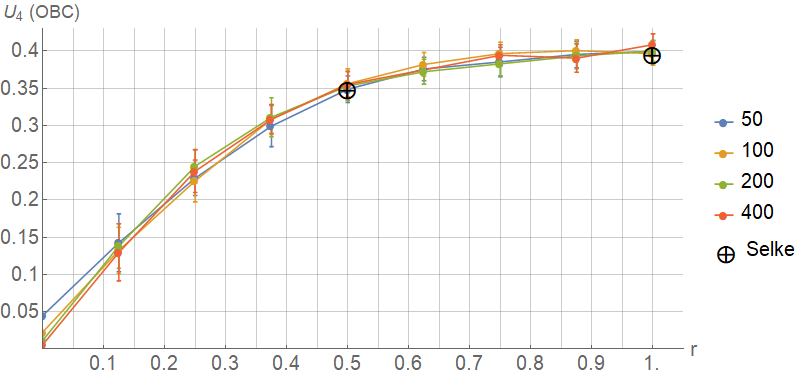
\includegraphics[width=100mm]{Sections/Images/CumulantOBC.png}
    \caption{График зависимости значения кумулянта Биндера в крит. точке от Aspect Ratio при открытых гран. условиях}
    \label{fig:CumulOBC}
\end{figure}

\begin{figure}[!h]
    \centering
    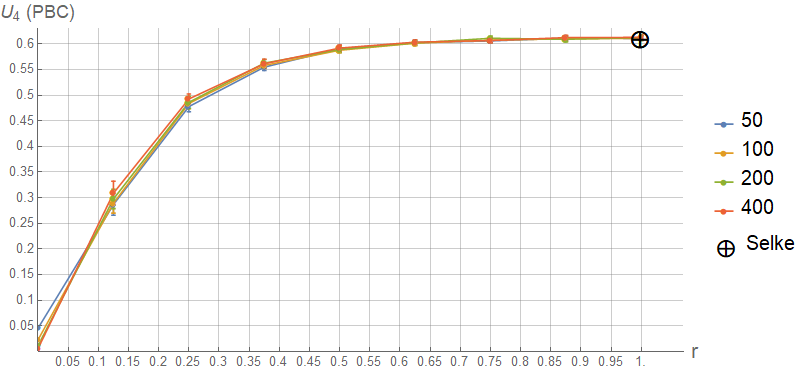
\includegraphics[width=100mm]{Sections/Images/CumulantPBC.png}
    \caption{График зависимости значения кумулянта Биндера в крит. точке от Aspect Ratio при периодических гран. условиях}
    \label{fig:CumulPBC}
\end{figure}

Крайние левые точки в отметке нуля являются расчётами для модели одномерного Изинга (где длина цепочки равна соответствующей стороне в двумерном изинге). Так, в случае открытых гран. условий (рис. \ref{fig:CumulOBC}) и периодических (рис. \ref{fig:CumulPBC}) значения кумулянта стремится к нулю с увеличением длины цепочки(см. Проект6.pdf\cite{Git}).
Черными точками отмечены значения критического кумулянта из работы Уолтера Сельке - 0.396 ± 0.002 для квадратной модели и 0.349 ± 0.002 для прямоугольной с отношением сторон r = 1/2 при открытых гран. условий. Для периодического случая квадратной модели критический кумулянт равен 0.61069\cite{Selke}.

Эти же значения отмечены в графиках \ref{fig:CumulOBCL} и \ref{fig:CumulPBCL} зависимости крит. кумулянта от обратной длины стороны как крайние левые (в нуле - так обозначен случай термодинамического предела).

\begin{figure}[!h]
    \centering
    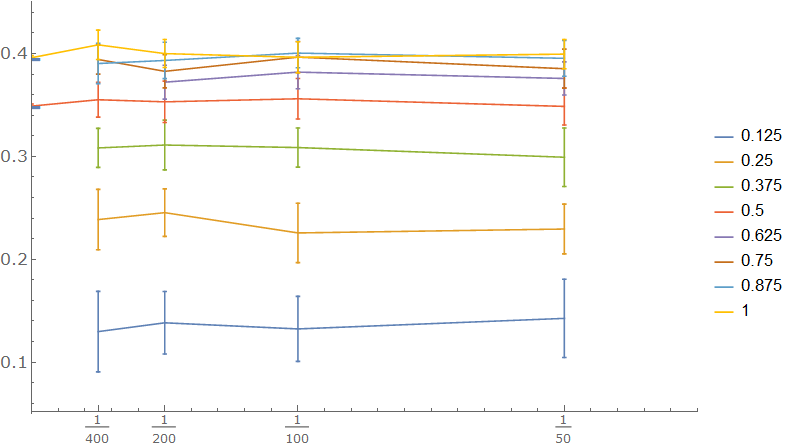
\includegraphics[width=100mm]{Sections/Images/CumulantOBCL.png}
    \caption{График зависимости значения кумулянта Биндера в крит. точке от обратной длины стороны при открытых гран. условиях}
    \label{fig:CumulOBCL}
\end{figure}

\begin{figure}[!h]
    \centering
    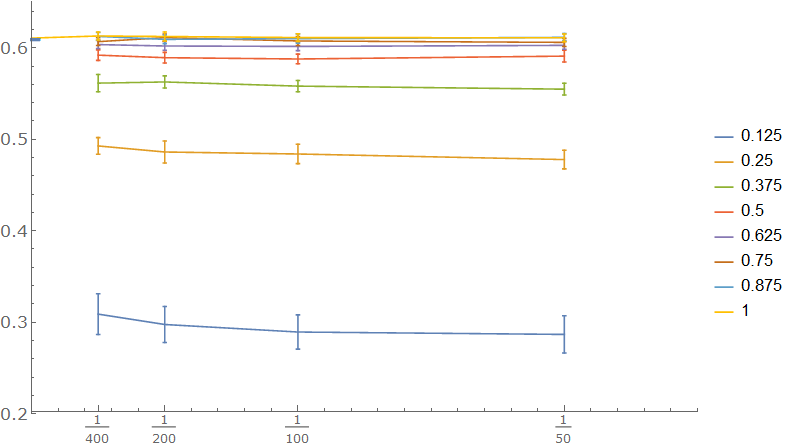
\includegraphics[width=100mm]{Sections/Images/CumulantPBCL.png}
    \caption{График зависимости значения кумулянта Биндера в крит. точке от обратной длины стороны при периодических гран. условиях}
    \label{fig:CumulPBCL}
\end{figure}

Учитывая погрешность в расчётах симуляций, зависимость от обратной длины прямоугольника 1/L не наблюдается.

\subsection{Сравнение модели Изинга и модели взаимодействующих непересекающихся блужданий}

Здесь мы рассмотрим основные понятия в модели взаимодействующих блужданий (Self-Avoiding Walks, SAWs), связанные с их формой и сравним их с прямоугольной моделью в тех же условиях. 

Важнейшим параметром в описании полученной симуляциями Монте-Карло блуждания является радиус инерции, численно равный среднему квадратическому расстоянию частиц от положения среднего арифметического центра модели (сумма $w_{k}$ в скобке)\cite{Pelissetto}:

\begin{equation}\label{eq:Rg}
    R^{2}_{g} = \frac{1}{N+1} \sum^{N}_{i=0}\left(w_{i} - \frac{1}{N+1}\sum^{N}_{k=0}w_{k}\right)^2 = \frac{1}{2(N+1)^{2}}\sum^{N}_{i,j=0}(w_{i} - w_{j})^{2}
\end{equation}

Так же для описания формы модели применяется тензор вращения относительно центра масс - матрица, $\alpha\beta-$й элемент которой расчитывается по формуле (4) из статьи\cite{Janke_G} :

\begin{equation}\label{eq:Ten_G1}
    Q_{N,\alpha\beta} = \frac{1}{N+1} \sum^{N}_{i=0}(w_{i,\alpha} - w_{c, \alpha})(w_{i,\beta} - w_{c, \beta})
\end{equation}
где $w_{c,\alpha} - \alpha$ -я координата вектора центра масс. В случае, если начало координат расположено в центре масс (следовательно, сумма векторов точек блуждания = 0), формула $\alpha\beta-$элемента тензора упрощается и численно равна второму моменту координаты (если $\alpha = \beta$), или до среднего произведения разных координат по всем точкам блуждания.


\begin{align}\label{eq:Ten_G_C}
    Q_{N,\alpha\beta} = &\frac{1}{(N+1)} \sum_{i=0}^{N} w_{i, \alpha} w_{i, \beta} \\
    \sum^{N}_{i=0}w_{i} &= 0
\end{align}

Рассмотрим формулу \eqref{eq:Ten_G1}. Так так $w{c}$ - центра масс блуждания, то:

\begin{equation}
    w_{c} = \frac{1}{N+1} \sum_{k=0}^{N} w_{k}
\end{equation}

Так же можно представить i-й вектор блуждания как:

\begin{equation}
    w_{i} = \frac{1}{N+1} \sum_{k=0}^{N} w_{i}
\end{equation}

Это позволит нам вытащить из скобок N+1 и избавиться от неизвестного $w_{c}$

\begin{align*}
    Q_{N,\alpha\beta} = \frac{1}{(N+1)^{3}} \sum^{N}_{i=0}(\sum^{N}_{k=0}(w_{i,\alpha} - w_{k, \alpha}))(\sum^{N}_{l=0}(w_{i,\beta} - w_{l, \beta})) = \\
    = \frac{1}{(N+1)^{3}} \sum^{N}_{i=0} \sum^{N}_{k,l=0}(w_{i,\alpha} - w_{k, \alpha})(w_{i,\beta} - w_{l, \beta}) = \\
    \frac{1}{(N+1)^{3}} \sum^{N}_{i=0} \sum^{N}_{k,l=0} (w_{i,\alpha} w_{i,\beta} - w_{i,\alpha} w_{l,\beta} - w_{k,\alpha} w_{i,\beta} + w_{k,\alpha} w_{l,\beta})
\end{align*}

Расскроем суммирование у учётов зависимостей индексов:

\begin{align*}
    Q_{N,\alpha\beta} = \frac{1}{(N+1)^{2}} (\sum^{N}_{i,k=0}(w_{i,\alpha} w_{i,\beta}) - \sum^{N}_{i,l=0}(w_{i,\alpha} w_{l,\beta}) - \sum^{N}_{i,k=0}(w_{k,\alpha} w_{i,\beta}) + \sum^{N}_{k,l=0}(w_{k,\alpha} w_{l,\beta})) = \\
    \frac{1}{(N+1)^{2}} \sum^{N}_{i,k=0}(w_{i,\alpha} w_{i,\beta} - w_{k,\alpha} w_{i,\beta}) = \frac{1}{2(N+1)^{2}} \sum^{N}_{i,k=0}(w_{i,\alpha} - w_{k, \alpha})(w_{i,\beta} - w_{k, \beta})
\end{align*}
т.к. кол-во произведений координат разных векторов и одинаковых меньше в два раза. Полученная формула:

\begin{equation}\label{eq:Ten_G2}
    Q_{N,\alpha\beta} \frac{1}{2(N+1)^{2}} \sum^{N}_{i,k=0}(w_{i,\alpha} - w_{k, \alpha})(w_{i,\beta} - w_{k, \beta})
\end{equation}

совпадает с формулой (4.1) из статьи о взаимодействующих блужданиях\cite{Pelissetto}, что значит что используемое ими понятие "тензора вращения" совпадает.

\subsection{Тензор инерции и тензор вращения}

Можно заметить некоторое сходство в расчётах недиагональных элементов тензора инерции J и тензора вращения из статей\cite{Pelissetto, Yanke_G}. Действительно, для системы из N материальных точек единичной массы тензор инерции в системе центра масс рассчитывается следующим образом:

\begin{equation}
    J = \left(
    \begin{array}{ccc}
        J_{xx} & J_{xy} & J_{xz}  \\
        J_{yx} & J_{yy} & J_{yz} \\
        J_{zx} & J_{zy} & J_{zz}
    \end{array} \right)
\end{equation}

\begin{align}
    J_{xy} &= J_{yx} = -\sum_{i=1}^{N} x_{i} y_{i} \\
    J_{yz} &= J_{zy} = -\sum_{i=1}^{N} y_{i} z_{i} \\
    J_{xz} &= J_{zx} = -\sum_{i=1}^{N} x_{i} z_{i} 
\end{align}

В тоже время, формулы диагональных элементов принципиально отличаются:

\begin{align}
    J_{xx} &= \sum_{i=1}^{N} y_{i}^{2} + z_{i}^{2} \\
    J_{yy} &= \sum_{i=1}^{N} x_{i}^{2} + z_{i}^{2} \\
    J_{zz} &= \sum_{i=1}^{N} x_{i}^{2} + y_{i}^{2}
\end{align}

Сравнивая с формулой элементов тензора вращения в системе центра масс \eqref{eq:Ten_G_C}, можно заметить, что недиагональные элементы тензоров отличаются знаком и усреднением в тензоре вращения. Диагональные же элементы "противоположны" друг другу:
в тензоре инерции они обозначают осевые моменты инерции (относительно $O\alpha$, и поэтому обозначенные моменты одной координатой ($J_{\alpha\alpha}$ используют сумму квадратов отличных от $\alpha$ координат.

Таким образом, элементы тензора вращения в системе центра масс в трехмерном простанстве можно представить как:

\begin{equation}
   Q_{\alpha\alpha} = \frac{1}{N}\sum^{N}_{i=1}w_{i,\alpha}^2 = \frac{1}{N} \left(\sum_{i=1}^{N}x_{i}^{2} + y_{i}^{2} + z_{i}^{2} - J_{\alpha\alpha}\right) = R^{2}_{g} - \frac{1}{N} J_{\alpha\alpha}  
\end{equation}

где $w_{i,\alpha}$ - $\alpha$-я координата радиус-вектора i-й материальной точки.

\begin{equation}
    Q_{\alpha\beta} = -\frac{1}{N} J_{\alpha\beta},\ \ \alpha \neq \beta
\end{equation}

Тогда матричный вид формулы тензора вращения через тензор инерции будет:

\begin{equation}
    Q = R_{g}^{2} * E - \frac{1}{N} J
\end{equation}
где E - это единичная матрица порядка, совпадающим с размерностью данной модели Dim.

Мы знаем, что симметричная матрица (какой являются и Q, и J) всегда диагонализируема, а базис из собственных векторов - ортогонален. Пусть S - матрица перехода в жорданов базис тензора инерции. Произведём переход в этот базис для тензора вращения:

\begin{equation*}
    S^{T}QS = S^{T} (R_{g}^{2} * E - \frac{1}{N} J) S = R^{2}_{g} * S^{T}ES-\frac{1}{N} * S^{T}JS
\end{equation*}

Матрица S - ортогональна, следовательно $S^{-1} = S^{T}$, поэтому:

\begin{equation}
    S^{T}QS = R^{2}_{g} * E - \frac{1}{N} * J_{D}
\end{equation}

где $J_{D}$ - диагонализированная матрица тензора инерции. Очевидно, что полученная в правой части матрица - диагональная. Следовательно, матрица в левой части так же получилась диагональной полсе перехода в новый базис и жорданов базис тензоров инерции и вращения одинаковы, пусть и с разными собственными значениями. Соответствующие собственные значения матриц в жордановом базисе будут равны:

\begin{align*}
    (S^{T}QS)_{ii} = Q_{D, ii} = R^{2}_{g} - \frac{1}{N}J_{ii},\ \ i=1..Dim
\end{align*}

Стоит подчеркнуть, что если жорданов базис составлен так, что собственные значения тензора инерции в матрице упорядочены по неубыванию, то в тензоре вращения собственные значения в матрице в этом базисе же будут упорядочены по невозрастанию.

\subsection{Показатели формы блуждания из тензора вращения}

Так как полученная матрица симметричная, то существует такой поворот, преобразующий её в диагональную (т.е., приводящий систему в Жорданов базис с собственными значениями по диагонали, и нулевыми недиагональными элементами), причём так, чтобы значения на диагонали были положительными и упорядоченными по невозрастанию.

В нашем двумерном случае, 

\begin{equation*}
    Q_{N} = \left(
    \begin{array}{cc}
      q_{1} & 0 \\
      0 & q_{2}
    \end{array} \right),\ 0 < q_{2} \leq q_{1}
\end{equation*}

Отметим так же, что сумма диагональных элементов тензора вращения равна квадрату радиуса вращения и инвариантна. Тогда определим ещё один показатель формы:

\begin{align*}
    s_{1} &= \frac{\la q_{1} \ra_{N}}{\la R_{g}^{2} \ra_{N}}\\
    s_{2} &= 1 - s1 = \frac{\la q_{2} \ra_{N}}{\la R_{g}^{2} \ra_{N}}\\
    r12 &= \frac{s1}{1-s1}
\end{align*}

Учитывая, что в $s_{1}$ и $s_{2}$ значения в числителе и знаменателе являются квадратами средних квадратичных значений, то следует вывод, что $\sqrt{r_{12}}$ является знакомым нам отношением сторон из предыдущего подраздела, только в данном случае это отношение не сторон прямоугольника, а полуосей эллипса инерции, который образует полученая симуляциями модель-блуждание.

\begin{figure}
\begin{minipage}[h]{0.5\linewidth}
     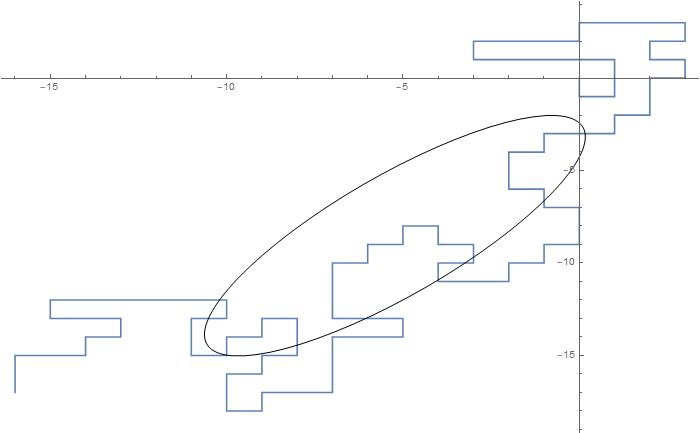
\includegraphics[width=\linewidth]{Sections/Images/GyrationEllipse.png}
\end{minipage}
\hfill
\begin{minipage}[h]{0.5\linewidth}
    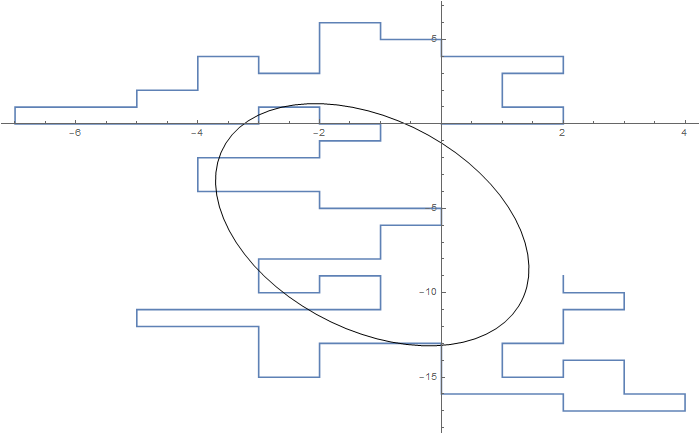
\includegraphics[width=\linewidth]{Sections/Images/GyrationEllipse2.png}
\end{minipage}
\vfill
\begin{minipage}[h]{0.5\linewidth}
     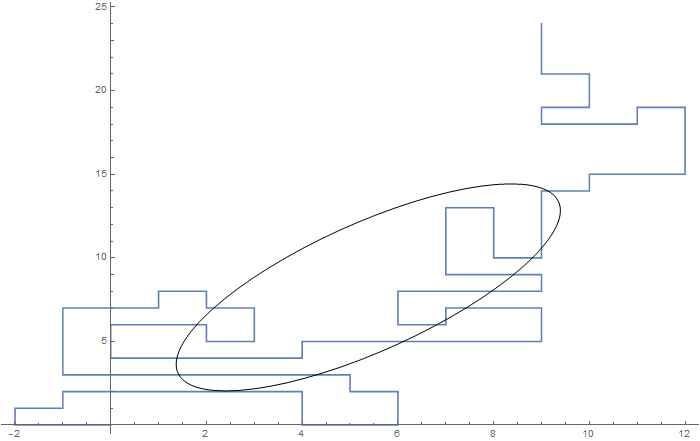
\includegraphics[width=\linewidth]{Sections/Images/GyrationEllipse3.png}
\end{minipage}
\hfill
\begin{minipage}[h]{0.5\linewidth}
    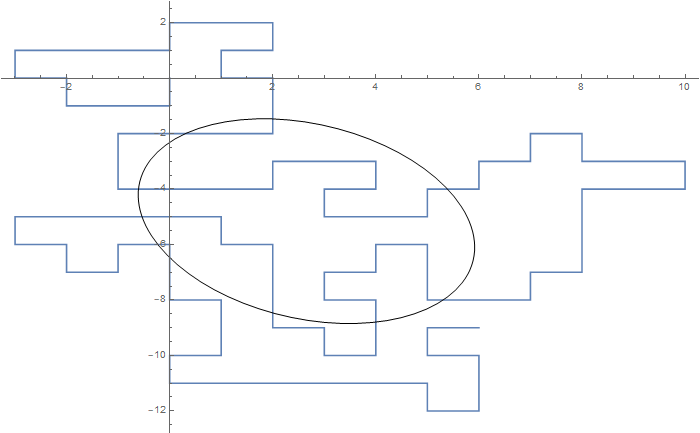
\includegraphics[width=\linewidth]{Sections/Images/GyrationEllipse4.png}
\end{minipage}
    \caption{Примеры работ симуляции по коду из Проект9.pdf\cite{Git}}
    \label{fig:my_label}
\end{figure}


\section{Геометрические свойства модели Изинга с точки зрения числа соседей в узлах}

\subsection{Сравнение модели Изинга и полимерной цепочки в решетках с 2-6 возможными соседями у мономеров}

\begin{figure}
    \centering
    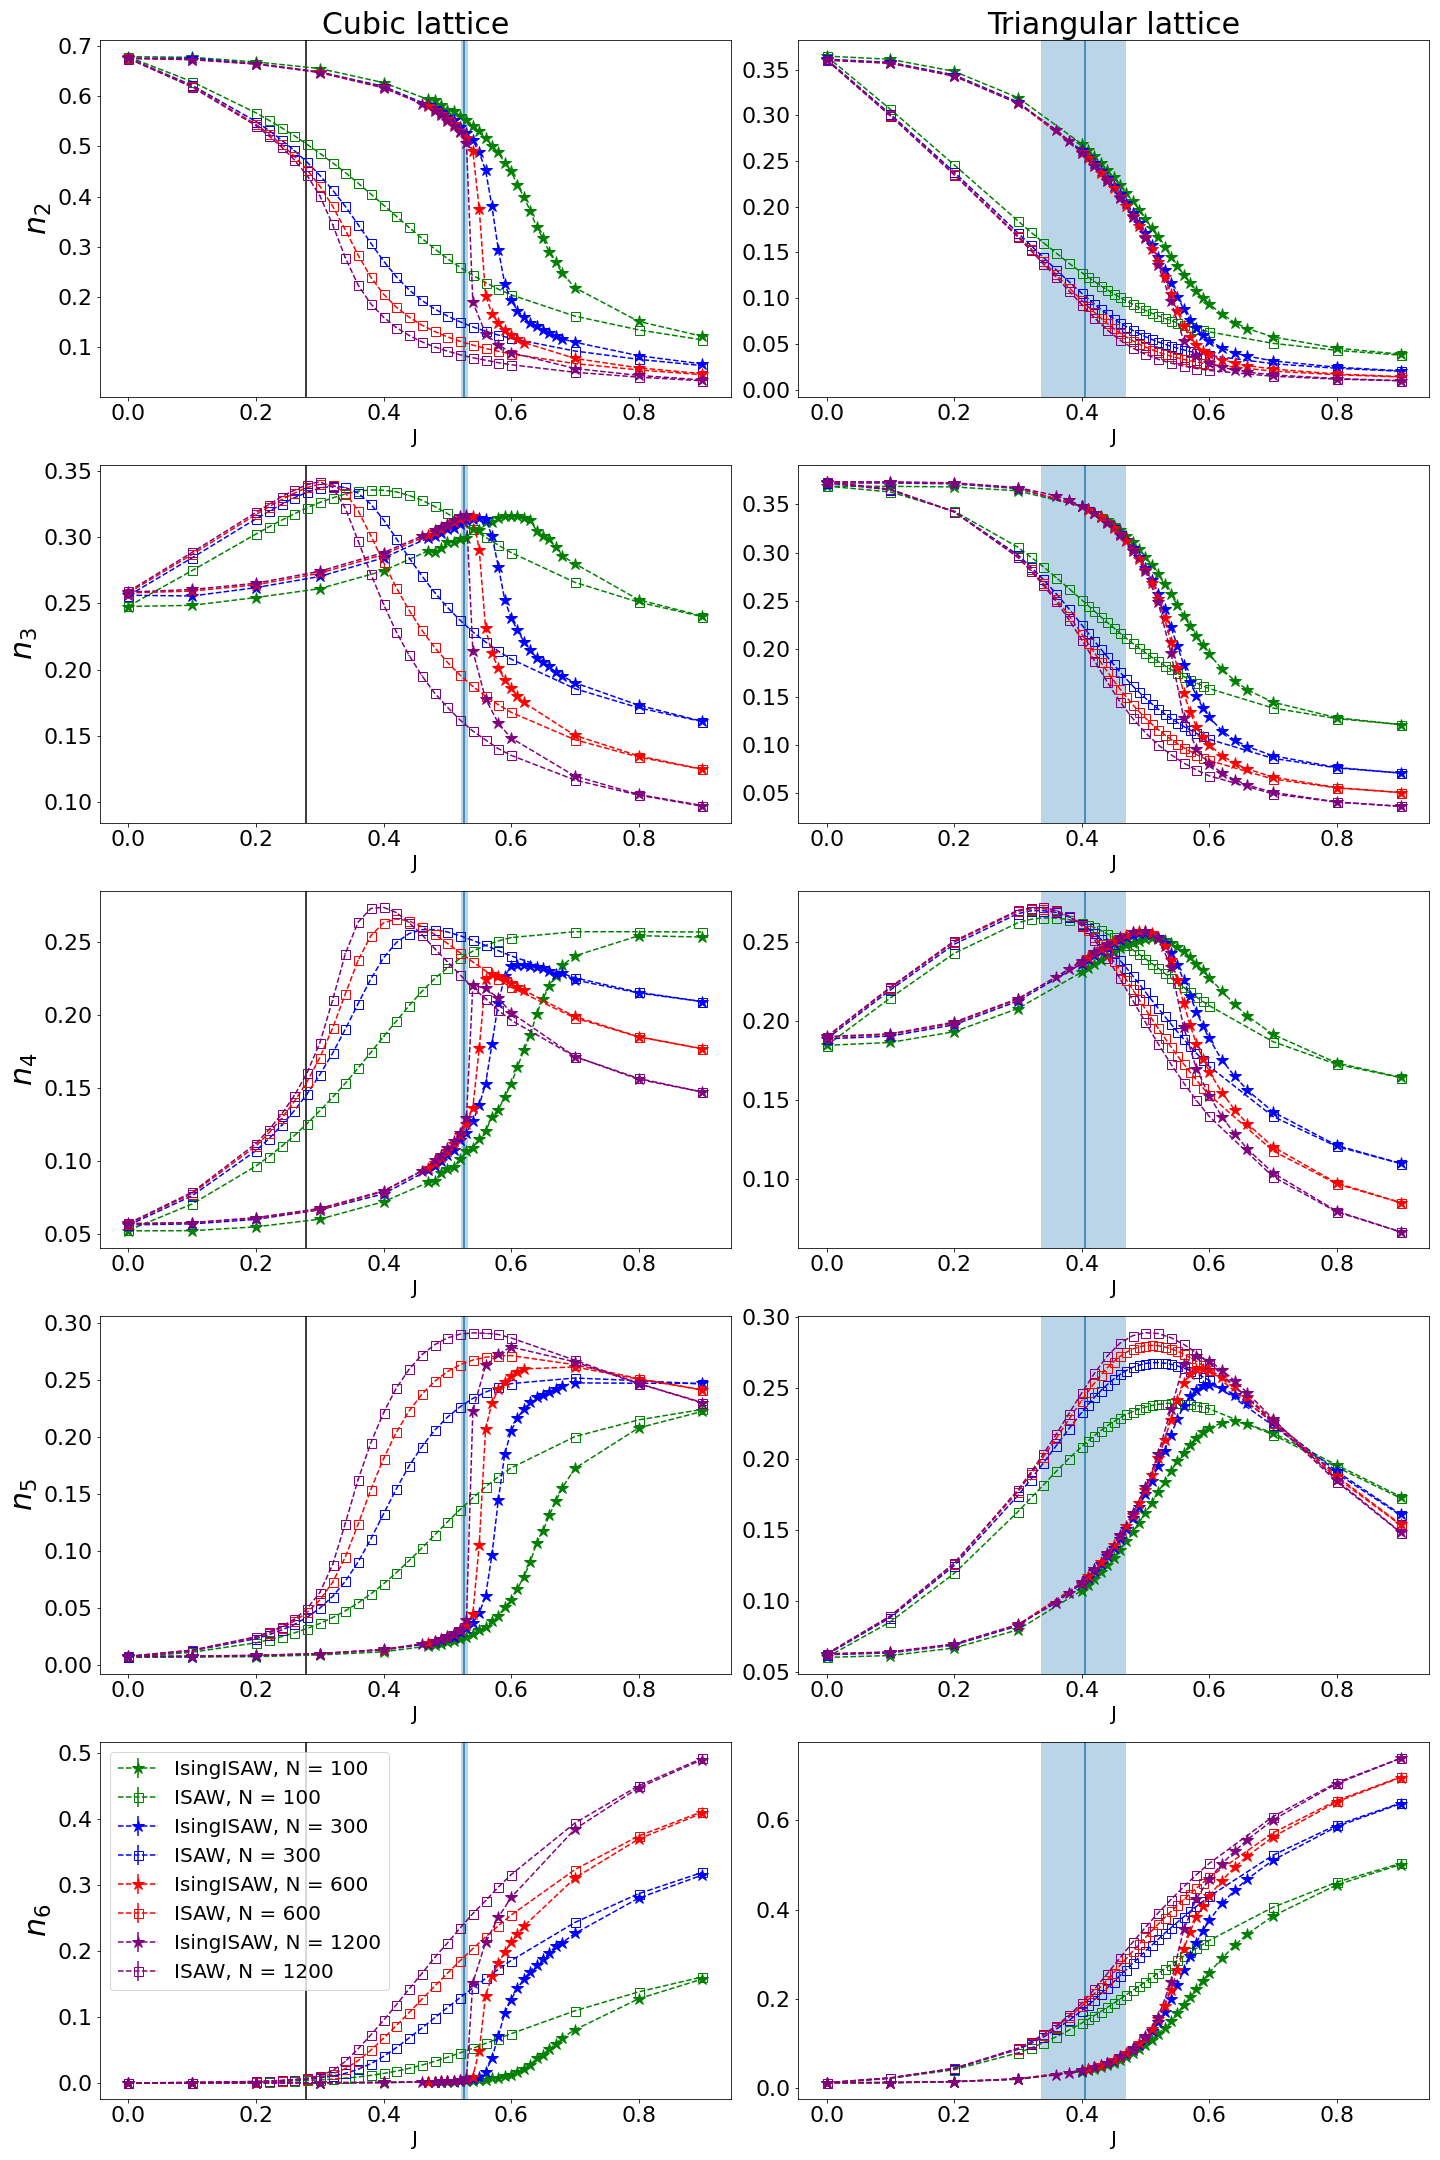
\includegraphics[width=0.95\textwidth, height=21.5cm]{Sections/Images/Ising_vs_ISAW.png}
    \caption{Fractions of monomers of Ising-ISAW model (stars) and ISAW model (open squares) on a cubic lattice (left column) and 2D-triangle lattice (right column) with 2-6 nearest neighbors as function of $J$ with length of conformations $N = $ 100 (green), 300 (blue) and 600 (red). Vertical lines define points of $\theta$-transition (For cubic lattice: black line for ISAW model \cite{Tesi1996} and blue line for Ising-ISAW model \cite{Foster2021}; for triangle lattice: blue line for ISAW model \cite{Privman1986})}
    \label{fig:Ising_vs_ISAW}
\end{figure}

\newpage

\subsection{Сравнение геометрических свойств модели Изинга на треугольной решётке с квадратной}

\begin{figure}
    \centering
    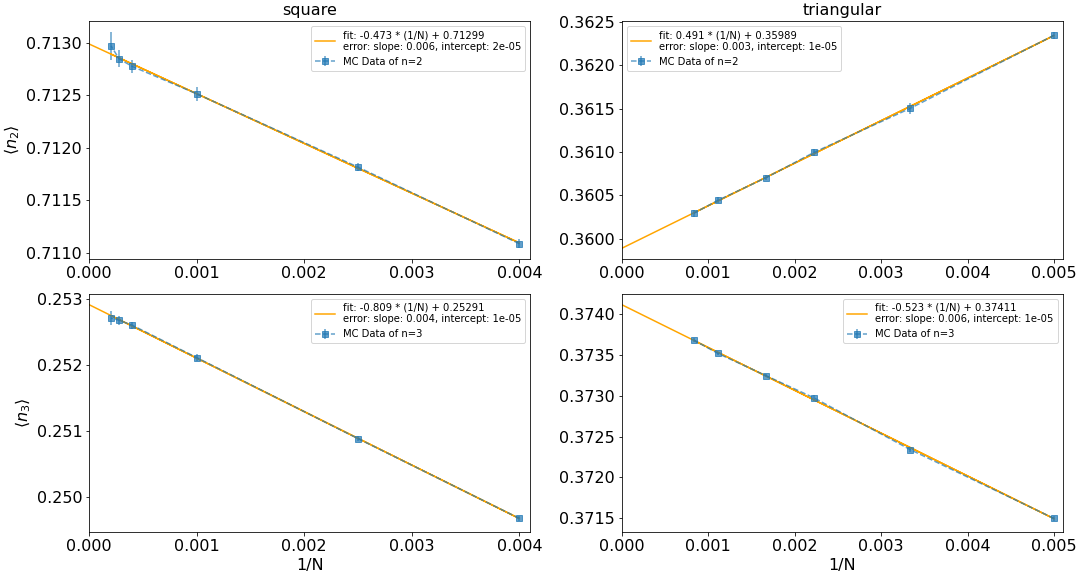
\includegraphics[width=0.95\textwidth]{Sections/Images/triagle_vs_square_bulk.png}
    \caption{Графики зависимости средней доли узлов с 2-3-мя соседями (сверху вниз) от обратной длины 1/N в модели Изинга на треугольной (слева) при N от 200 до 1200 и квадратной (справа) решётках при N от 250 до 4900 при J=0. Синяя линия описывает результаты симуляций Монте-Карло, оранжевая - линейное приближение результатов, ошибки рассчитаны с учётом погрешностей полученных данных}
    \label{fig:tr_vs_sq_bulk}
\end{figure}

На графике \ref{fig:tr_vs_sq_bulk} наглядно показано сравнение приближений долей "одномерных" участков (то есть, долей мономеров с двумя соседями) и узлов с тремя соседями в цепочках на треугольной и квадратной решётках. Для расчётов долей на треугольной решётке были использованы длины 200-1200, для квадратной - 250-4900. Приближение долей треугольной решётки имеет отчётливый линейный характер, включая даже в приближении на всех точках (см. раздел "Подсчёт соседей у треугольной решётки" в Bulk2-6.ipynb\cite{Git}). Линейность долей квадратной решётки также подтверждается (с учётом погрешности расчётов с наибольшей длиной).

Так же хочется заметить некоторое сходство значений свободного члена для долей с двумя соседями и свободного члена в приближениях графика зависимости вероятности гомополимерной цепочки иметь атмосферу 3 в статье Преллберга\cite{Prellberg}, то есть вероятность, что второй конец цепочки длины N имеет 3 возможных направления для удлинения и следовательно, 3 узла, которые могут стать N+1-ым в цепочке.

\begin{table}[]
    \centering
    \begin{tabular}{|c|c|c|c|}
    \hline
    k & $p^{(k)}$ & i & $intercept(\la n_{i} \ra)$ \\ \hline
    3 & 0.711 14(3) & 2 & $0.71299 \pm 2*10^{-5}$ \\ \hline
    2 & 0.225 00(2) & 3 & $0.25291 \pm 10^{-5}$ \\ \hline
    1 & 0.054 76(1) & 4 & $0.03410 \pm 10^{-5}$\\ \hline
    0 & 0.009 096(4) & - & - \\ \hline
    \end{tabular}
    \caption{Таблица сравнения свободных членов линейных приближений вероятностей у конформации иметь n-ю атмосферу (слева) и долей мономеров с i соседями (справа) в зависимости от обратной длины конформации 1/N}
    \label{tab:Prellb_Compare}
\end{table}

На таблице \ref{tab:Prellb_Compare} слева изображены значения свободных членов графика зависимости вероятности гомополимерной цепочки иметь атмосферу k в статье Преллберга\cite{Prellberg}, то есть вероятность, что второй конец цепочки бесконечно большой длины N имеет k возможных направления для удлинения и следовательно, k возможных узлов, которые могут стать новым узлом в цепочке. Справа изображены значения свободных членов приближений графиков долей узлов с i соседями. Хотя все значения отличаются больше чем на погрешность расчётов, однако нельзя не заметить довольно близкое сходство $p^{(3)}$ и свободного члена $\la n_{2} \ra$, хотя сами приближения имеют противоположные по знаку наклоны. 
Возможно, обе величины по-разному описывают одно и то же поведение цепочек с точки зрения их плотности: например, если конец цепочки длины N (назовём его "N-ым узлом") имеет атмосферу три, то при добавлении нового N+1-го узла N-й будет иметь два соседа: N-1-й и N+1-й узлы. Так же при атмосфере 2 (то есть, уже имея два соседа и две возможности для удлинения) N-ый узел при удлинении будет иметь 3 соседа. И наконец, при атмосфере 1 удлинение цепочки приведёт к тому, что старый конец цепочки будет иметь 4 соседа. Очевидно, что случай удлинения при атмосфере 0 рассмореть невозможно, и провести аналогию с соседями нельзя.

Однако сходства между одномерием треугольной и квадратной решётки с точки зрения самих приближений почти не наблюдается - они имеют как разные значения свободных членов, так и значения и даже (в случае 2-х соседей) знаки коэффициента наклона, разница который значительно превышает погрешность фита.



\subsection{Сравнение геометрических свойств модели Изинга на треугольной решётке с кубической}

\begin{figure}
    \centering
    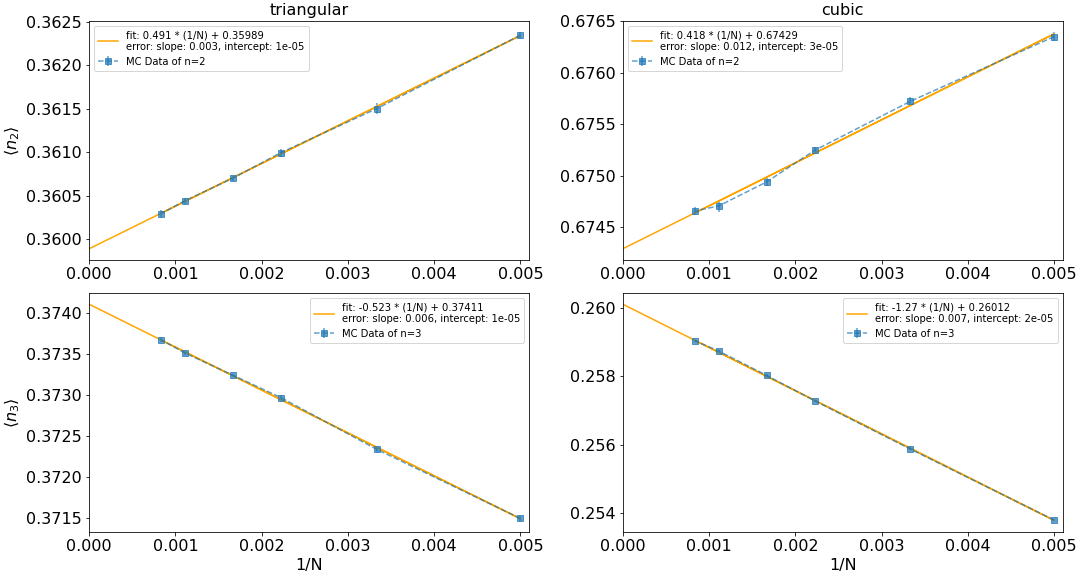
\includegraphics[width=0.95\textwidth]{Sections/Images/triangle_vs_cubic_bulk.png}
    \caption{Зависимость средней доли узлов с 2-3-мя соседями (сверху вниз) от обратной длины 1/N в модели Изинга на треугольной (слева) и кубической (справа) решётках при J=0. Синяя линия описывает результаты симуляций Монте-Карло, оранжевая - линейное приближение результатов, ошибки рассчитаны с учётом погрешностей полученных данных}
    \label{fig:tr_vs_cb_bulk}
\end{figure}

Здесь мы сравниваем линейное приближение треугольной решётки с кубической, имеющейтакое же количество возможных соседей. Получается примерно та же ситуация как и в случае сравнения с квадратной - кубическая решётка на графике \ref{fig:tr_vs_cb_bulk} показывает почти чёткий линейный характер приближения в пределах погрешности наибольших длин (для n=3 линейно видна значительно лучше), но значения не имеют никакого сходства. Единственное отличие от сравнения с квадратной решёткой - графики соответствующих долей имеют одинаковое поведение с точки зрения знака наклона, что действительно и для долей узлов с больший числом соседей. Можно утверждать, что треугольная решётка с точки зрения поведения доли одномерных участок больше похожа на кубическую решётку, нежели квадратную, однако универсальность поведения доли "одномерных" участков среди решёток при бесконечно больших длинах конформации не обнаружена.

\bibliographystyle{plain}
\bibliography{bibliography}

\end{document}



